\documentclass[a4paper]{article}

\usepackage{graphicx}
\usepackage{amsmath,amssymb}
\usepackage{minted}
\usepackage{multirow}
\usepackage{float}
\usepackage{todonotes}
\usepackage{forest}
\usepackage{xstring}
\usepackage{xcolor}
\usepackage[most]{tcolorbox}
\usepackage{xparse}

\usetikzlibrary{graphs,graphdrawing}
\usegdlibrary{layered}

% for external graphviz
\input{/home/donkarlo/Dropbox/repo/nd_ai_project/src/nd_ai/knoweldge_representation/language/formal/computer/programming/tex/latex/code_clips/external_graphviz.tex}

%for tags, comma separated \semtag{tag1, tag2}
\input{/home/donkarlo/Dropbox/repo/nd_ai_project/src/nd_ai/knoweldge_representation/language/formal/computer/programming/tex/latex/parts/control_sequence/kind/semtag/semtag.tex}

% for links, just type \seehere
\input{/home/donkarlo/Dropbox/repo/nd_ai_project/src/nd_ai/knoweldge_representation/language/formal/computer/programming/tex/latex/code_clips/seehere.tex}

\title{}
\date{}

\begin{document}
    \maketitle
    \url{https://www.sciencedirect.com/science/article/abs/pii/S0028393209000645?via%3Dihub} says:
    There are essentially nine properties of episodic memory that collectively distinguish it from other types of memory. Other types of memory may exhibit a few of these properties, but only episodic memory has all nine:
    
    \begin{itemize}
        \item Contain summary records of sensory-perceptual-conceptual-affective processing.
        \item Retain patterns of activation/inhibition over long periods.
        \item Often represented in the form of (visual) images.
        \item They always have a perspective (field or observer).
        \item Represent short time slices of experience.
        \item They are represented on a temporal dimension roughly in order of occurrence.
        \item They are subject to rapid forgetting.
        \item They make autobiographical remembering specific.
        \item They are recollectively experienced when accessed.
    \end{itemize}
    
    \section{Definition of episodic and episode}
    Episodic Memory (EPMEM) automatically records snapshots of working memory in a temporal stream. Prior episodes can be retrieved into working memory through query. Once an episode has been retrieved, the next (or previous) episode can then be retrieved. An agent may employ EPMEM to sequentially play through episodes from its past (allowing it to predict the effects of actions), retrieve specific memories, or query for episodes possessing certain memory structures. \url{https://en.wikipedia.org/wiki/Soar_(cognitive_architecture)#Episodic_memory}
    
    Episodic memory is the memory of events and experiences that can be recalled in relation to a specific time and in proper order \cite{tulving-2002-episodic-memory-from-mind-to-brain}
    
    Endel Tulving originally described episodic memory as a record of a person's experience that held temporally dated information and spatio-temporal relations \cite{tulving-1983-elements-of-episodic-memory}.
    
    A feature of episodic memory that Tulving later elaborates on is that it allows an agent to imagine traveling back in time \cite{tulving-2002-episodic-memory-from-mind-to-brain}.
    
    In the 1972 paper Tulving stated that episodic memory
    "stores information about temporally dated episodes or events and temporal-
    spatial relations among these events" (p. 385) \cite{tulving-1972-episodic-and-semantic-memory}
    
    
    \section{Episode}
    \cite{tulving-2002-episodic-memory-from-mind-to-brain} defines episodes as integrated representations of events situated in a spatiotemporal context.
    
    \paragraph{Event} An event according to \cite{davidson-1969-the-individuation-of-events} Events are particular occurrences that can be described in terms of actions and their properties. Spatiotemporal is the association of location with time.
    
    \cite{morales-calva-2025-tell-me-why-the-missing-w-in-episodic-memorys-what-where-and-when} defines an eposide as it is shown in \ref{morales-calva-2025-tell-me-why-the-missing-w-in-episodic-memorys-what-where-and-when-figure-2}
        \begin{figure}[H]
            \centering
            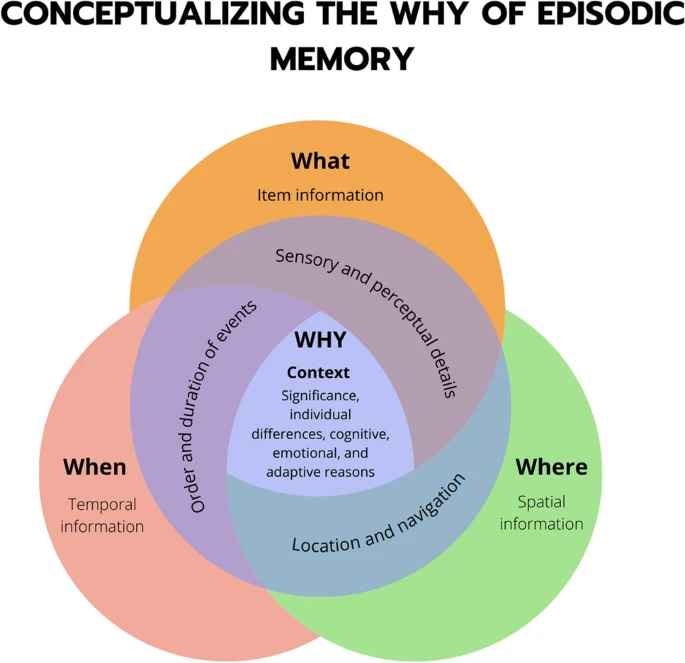
\includegraphics[width=0.5\textwidth]{morales-calva-2025-tell-me-why-the-missing-w-in-episodic-memorys-what-where-and-when-figure-2}
            \label{morales-calva-2025-tell-me-why-the-missing-w-in-episodic-memorys-what-where-and-when-figure-2}
            \caption{From \cite{morales-calva-2025-tell-me-why-the-missing-w-in-episodic-memorys-what-where-and-when} figure 2}
        \end{figure}
    \bibliographystyle{plain}
     \bibliography{/home/donkarlo/Dropbox/repo/nd_shared_research/bibliography/bibliography.bib}
\end{document}